\begin{frame}[parent={cmap:software-testing-foundations}, hasprev=false, hasnext=true]
\frametitle{Processo de teste de software}
\label{concept:software-testing-process}
\label{concept:test-process}

\begin{block:fact}{Processo de teste de software}
\begin{itemize}
	\item Quando realizada de forma sistemática e lúcida, o teste de software ajuda:
	\begin{itemize}
		\item Aumentar a confiança de que o produto se comporta de acordo com sua especificação;

		\item Destacar as características mínimas de qualidade do produto.
	\end{itemize}
\end{itemize}
\end{block:fact}
\end{frame}


\begin{frame}[hasprev=true, hasnext=false]
\frametitle{Conceitos de teste de software}
\framesubtitle{Teste de software}

\begin{block:fact}{}
	\centering
	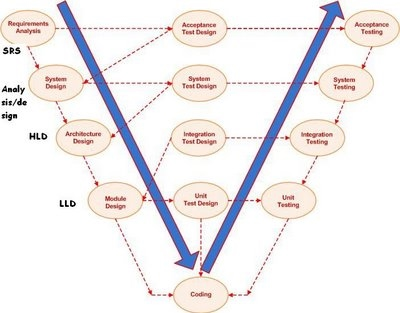
\includegraphics[width=8cm]{teste-de-software/conceitos-basicos/Imagens/v-model}
\end{block:fact}
\end{frame}